\documentclass[fr]{../../../../../../eplexam}

\hypertitle{Probabilité et Statistiques}{5}{FSAB}{1105}{2016}{Août}{All}
{BAC3 2015-2016}
{Anouar El Ghouch}

\section{/6}

\begin{enumerate}
\item Pour les Jeux Olympiques, on a besoin de 200 balles. La firme A en produit 120 avec un taux de défaillance de 5\% et la firme B produit les 80 restantes avec un taux de défaillance de 10\%. Lors d'un match, 3 balles se révèlent être défectueuses.

Quelle est la probabilité qu'au moins deux de ces balles aient été conçues par la firme B?

\begin{center}
    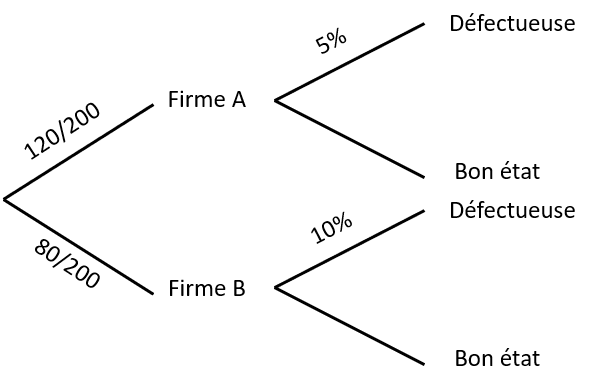
\includegraphics[scale=0.4]{Q1_1.png}
\end{center}

\item Je souhaite acheter une place pour aller voir les Jeux Olympiques. On m'a dit que la probabilité d'obtenir un billet en appelant au moins 3 fois est de 81\%.

Quelle est la probabilité que j'obtienne une place au deuxième coup de fil?

\item Dans un match de foot (90 min), le temps pour mettre le premier goal  suit une distribution exponentielle. La probabilité de mettre un goal à $2/3$ du match est de 90\%.

Quel est le temps moyen pour marquer le premier but?

\item Tu constates que la durée de connection de tes amis sur Facebook suit une loi uniforme entre 1 heure et 5 heures. Tu as 90 amis et tu veux savoir quelle est la probabilité que demain ils se connectent tous durant moins de 3 heures et 6 minutes en moyenne.
\end{enumerate}

\begin{solution}
\begin{enumerate}
\item Dénotons par $D$, le fait d'être défectueux. Cherchons d'abord la probabilité qu'une balle défectueuse ait été produite par la firme B.
$$P(B|D) = \frac{P(B \cap D)}{P(D)}=\frac{P(D|B)P(B)}{P(D|B)P(B)+P(D|A)P(A)}=\frac{0,4. 0,1}{0,4.0,1+0,6.0,05} = 0,571$$

Soit $X=$ le nombre de balles défectueuses produites par la firme B.
$X \sim Bi(3 ; p=0,571)$
$$P(X \geq 2) = P(X=2) + P(X=3) = C^2_3 \; p^2 (1-p) + C^3_3\;  p^3 = \boxed{0,6064}$$

\item Soit $X=$ le nombre d'appels réalisés avant d'avoir d'obtenu une place.
$X \sim Ge(p)$. 

Cherchons $p$. On sait que
\begin{eqnarray*}
P (X \geq 3) & = & 0,81 \\
& = & 1 - P(X < 3)\\
& = & 1 - P(X=1) - P(X=2)\\
& = & 1 - p(1-p) - p
\end{eqnarray*}

$$p^2 - 2p + 0,19 = 0$$
$$p=0,1 \;\;\; \textup{ou} \;\;\; 1,9 > 1 \;\;\; \textup{à rejeter}$$

Donc $$P(X=2) = p(1-p) = \boxed{0,09}$$
\item Soit $X=$ le temps moyen pour marquer le premier but [min].\\
$X \sim Expo(\beta)$. On cherche $\beta$.

On sait que 

$$P(X\leq\frac{2}{3}\cdot90)=0,90 = F(\frac{2}{3}\cdot90)$$

avec $F(x)=\displaystyle \int_0^x f(x) dx = \int_0^x \frac{1}{\beta} e^{\frac{-x}{\beta}} dx = 1 - e^{\frac{-x}{\beta}}$

Donc on a 
$$1-e^{\frac{-60}{\beta}}=0,90$$
$$\beta = \boxed{26 \; \textup{min}}$$

\item Notre grand échantillon d'amis Facebook permet au TCL de s'appliquer à la moyenne, on l'applique et on obtient
$$X\sim U[1,5] \qquad \mu = 3 \qquad \sigma^2 = \frac{4}{3}$$
On peut normaliser la distribution: 
$$X\sim N\left(3,\frac{4}{3}\right)\left(\frac{(X-\mu)\sqrt{n}}{\sigma}\right) $$
$$P(X<3.1) = 1-P(X>3.1) =1-P(Z>0.8216) = 0.79435$$ 
\end{enumerate}

\end{solution}


\section{/2}

Soit $X$ et $Y$ deux variables aléatoires. On sait que $X$ suit une distribution exponentielle avec une moyenne égale à 2. On ne connaît pas la distribution de $Y$ mais on sait que sa variance $Var(Y)=16$. On sait aussi que la corrélation $Corr(X,Y)=0.25$.

\begin{enumerate}[label=\alph*)]
    \item Trouver l'asymétrie de $X$ définie comme $Asym(X) = E\Big(\frac{(X-\mu)^3}{\sigma^3}\Big)$ avec $\mu=E[X]$ et $\sigma^2=V[X]$.
    \item Trouver la valeur du paramètre $a$ qui minimise $V(aX + (1 - a)Y)$.
\end{enumerate}

\begin{solution}

\begin{enumerate}[label=\alph*)]
    \item $X \sim Expo(\beta=2) \longrightarrow E(X)=2 \; ;\; V(X)=4$
    
    Puisque $E$ est un opérateur linéaire, on a 
    $$E\Bigg(\frac{(X-\mu)^3}{\sigma^3}\Bigg) = \frac{1}{\sigma^3}\Big(E(X^3)-3\mu E(X^2) + 3 \mu^2 E(X) - \mu^3\Big) = \boxed{2}$$
    
    avec 
    $$\sigma^3 = (\sigma^2)^{\frac{3}{2}} = 8$$
    $$E(X^2)=2\beta^2=8$$
    $$E(X^3)=6\beta^3=48$$
    
    Ici, on a utilisé la formule $\displaystyle \int_0^{\infty} x^n e^{-kx} dx = \frac{n!}{k^{n+1}}$ pour calculer les $E(X^n)$ sans devoir faire de l'intégration par partie. Il est aussi possible de les calculer via la moment generating function.
    
    
    \vspace{5mm}
    \item 
    $Corr(X,Y)= 0.25 = \frac{Cov(X,Y)}{\sqrt{V(X)V(Y)}} \Longrightarrow Cov(X,Y)= 0,25 \sqrt{4}\sqrt{16}=2$
    \begin{eqnarray*}
    V(aX + (1 - a)Y) & = &  a^2 V(X) + (1-a)^2 V(Y) + 2a(1-a) Cov(X,Y)\\
    & = & a^2 (4+16-2\cdot2) + a(-2\cdot16+2\cdot2) +16\\
    & = & 16a^2 -28a +16
    \end{eqnarray*}
    
    $$\frac{dV}{da} = 0 = 32a -28 \Longrightarrow \boxed{a=\frac{7}{8}}$$
    
\end{enumerate}

\end{solution}


\section{/5}
Soit $X_1, X_2, \ldots, X_n$ des variables aléatoires distribuées de manière iid avec avec une fonction de densité
\begin{align*}
f(x, \theta)=
\begin{cases}
    (\theta+1)x^\theta  &  0 \le x \le 1\\
    0 & \textup{ailleurs}
\end{cases}
\end{align*}
avec $\theta >-1$.

\begin{enumerate}[label=\alph*)]
    \item Trouver le maximum de vraisemblance de $\theta$, qu'on va noter $\hat{\theta}_{MV}$.
    \item Montrer que $Z = -\ln(X)$ suit une distribution de type exponentielle avec pour moyenne $\beta=(\theta+1)^{-1}$.
    \item Est-ce que $\hat{\theta}_{MV}$ est biaisé? Si oui, trouver un estimateur non biaisé.
    \item Déduire le maximum de vraisemblance de $E[X]$.
    \item Donner la distribution asymptotique de $\hat{\theta}_{MV}$.
\end{enumerate}

\begin{solution}

\begin{enumerate}[label=\alph*)]
    \item  On doit maximiser $L(\theta)$
    
    \begin{eqnarray*}
    L(\theta) & = &  \prod_i^n f(x_i,\theta) \qquad \textrm{car $X_i$ indépendants} \\
    & = & (\theta + 1)^n \prod_i^n x_i^\theta
    \end{eqnarray*}
    On applique le $\ln$. Puisque c'est une fonction strictement croissante, maximiser $L(\theta)$ ou $\ln(L(\theta)) \equiv LL(\theta) $, c'est identique.
    $$LL(\theta) = n \;\ln (\theta +1) + \theta \sum_i^n \ln(x_i)$$
    On dérive et on égale à $0$.
    
    $$\frac{dLL(\theta)}{d\theta}\Bigg|_{\theta=\Hat{\theta}} = \frac{n}{\Hat{\theta} +1} + \sum_i^n \ln(x_i) = 0$$
    $$\boxed{\Hat{\theta} = - \Bigg( 1+\frac{1}{\overline{\ln{x}}} \Bigg)}$$
    
    Il reste à vérifier que c'est bien un maximum et donc que sa dérivée seconde est négative. Ce qui est bien le cas.
    $$\frac{d^2LL(\theta)}{d\theta^2}\Bigg|_{\theta=\Hat{\theta}} = \frac{-n}{(\Hat{\theta}+1)^2}<0$$
    
    \item On applique la méthode des transformations avec $Z=g(X) = -\ln X$.
    
    $$f_Z(z)=\frac{f_X(x)}{|g'(x)|}\Bigg|_{x=g^{-1}(z)} = \frac{(\theta +1)x^{\theta}}{|\frac{1}{x}|}\Bigg|_{x=e^{-z}} = (\theta+1) e^{-z(\theta+1)}  \;\;\; \textup{avec} \; 0 \leq z \leq \infty $$
    
    On voit que $Z \sim Expo\big((\theta+1)^{-1}\big)$.

    \item 
    
    \item 
    
    \item 
\end{enumerate}
    
\end{solution}


\section{/3}
La société Test Achat prétend qu'en achetant le package A, le consommateur économise \textbf{au moins} 900 euros en moyenne par rapport à un même package A, acheté chez un concurrent.

\begin{enumerate}[label=\alph*)]
    \item On souhaite construire un intervalle de confiance de $98\%$ de longueur $12$ ($=\theta_U - \theta_L$). Chercher le nombre de consommateurs requis $n$, pour que l'étude que l'on a réalisée qui a fourni un écart-type de 40, soit cohérente.
    
    \item On fait une deuxième étude, cette fois on demande à 135 personnes. On obtient une moyenne d'économie de 910 euros, avec un écart-type de 50 euros. Qu'est-ce qu'on en déduit de Test Achat? Proposez un test d'hypothèse (bien préciser les hypothèses) avec $\alpha=5\%$. Quelle est la région de rejet? Quelles sont les conclusions sur base de la région de rejet?
    
    \item Quelle est la p-value de votre test d'hypothèse du point b? Quelles sont vos conclusions?
\end{enumerate}

\begin{solution}
\begin{enumerate}[label=\alph*)]
    \item  On fait l'hypothèse que la distribution peut être approximée par une normale.
    $$12 = 2\,z_{0,01} \frac{\sigma}{\sqrt{n}}$$
    $$\boxed{n \geq 240}$$
    
    \item 
    
    \item $$p-value = P(Z>2.32379) = 0.0103 < 0.025/0.05 $$
\end{enumerate}
\end{solution}


\section{/4}

On a $Y_1$ et $Y_2$ qui sont des variables aléatoires indépendantes de distribution uniforme dans l'intervalle [$\theta,\theta+1$].

\begin{enumerate}[label=\alph*)]
    \item Pour $\theta=0$, calculer $P(Y_1Y_2\ge \frac{1}{2}|Y_2\ge \frac{3}{4})$.
    
    \item Pour $\theta=0$, montrer que la fonction de densité de $U = Y_1 + Y_2$ vaut bien
    \begin{align}
    f_U(u)=
    \begin{cases}
    u,  &  0 \le u \le 1,\\
    2 - u, &  1 < u \le 2,\\
    0 & \mathrm{sinon}
    \end{cases}
    \end{align}
    
    \item On a $H_0: \theta=0$ et $H_a: \theta>0$. On fait deux tests: le premier où $H_0$ est rejeté si $Y_1>0.95$; le second où $H_0$ est rejeté si $Y_1 + Y_2 > c$. Chercher $c$ pour que les deux tests aient la même probabilité de commettre une erreur de type I.
\end{enumerate}

\begin{solution}

\begin{enumerate}[label=\alph*)]
    \item $$\int^1_{0,75} \int^1_{\frac{1}{2y}}1 \: \dif x\dif y=0.10615$$

    $P(A|B) = \frac{P(A \cup B)}{P(B)}$, donc il faut encore diviser ce résulat par $P(Y_2\ge \frac{3}{4})$ et on obtient 0.4246.
    
    \item
    
    \item  $c=1.6838$. Il suffit de calculer la probabilité que $Y_1$ soit supérieur à $0,95$, et ensuite trouver la cumulative $F_U(u) = -\frac{u^2}{2} + 2u - 1$.
\end{enumerate}

\end{solution} 

\end{document}
